\subsection{Framework Overview}
\label{subsec:framework}

HP-PDHG is organized around a four-stage core loop. A population of primal-dual states first evolves under PDHG on the continuous relaxation. Selected members then undergo a barrier-aware non-local perturbation step inspired by WKB-style tunneling. At prescribed intervals, a progressive integrality-projection operator softly pushes integer-constrained coordinates toward the lattice. Finally, promising candidates are passed to a feasibility-aware repair routine before they can replace the incumbent solution. The resulting separation of roles is deliberate: PDHG provides stable relaxation dynamics, non-local perturbation broadens exploration, projection contracts non-integrality, and repair protects feasibility. In the current mainline implementation, this core loop can further be overlaid with an optional feasibility-first two-phase controller that changes how strongly constraints are emphasized over time. For continuity with stored result files, the implementation label \emph{Quantum Pop-PDHG} is retained in some tables and artifacts, but it refers to the same HP-PDHG solver described here.

\begin{figure}[htbp]
    \centering
    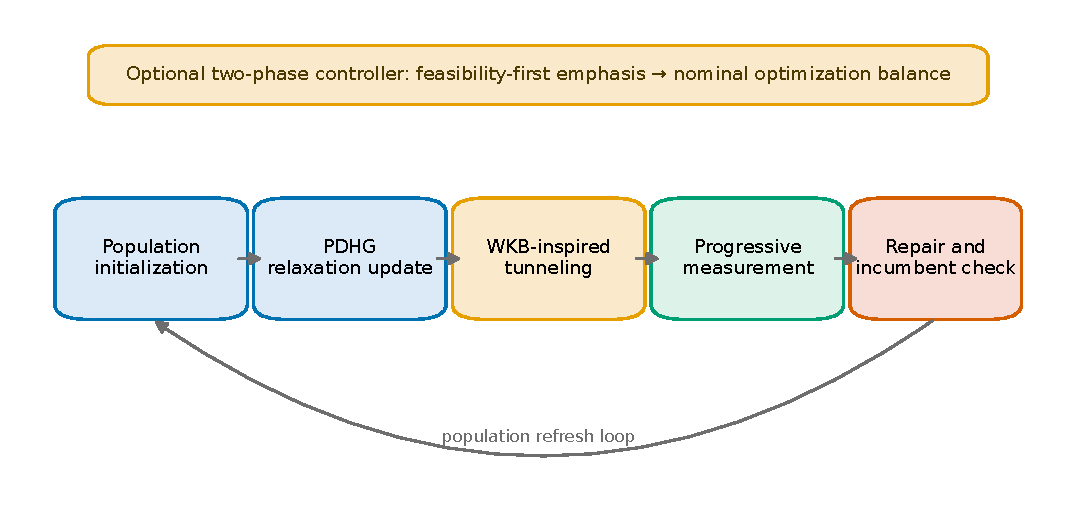
\includegraphics[width=0.82\textwidth]{figures/framework_overview_nature.pdf}
    \caption{Overview of the HP-PDHG workflow. The figure highlights the information flow from relaxation search to incumbent update and clarifies the distinct roles of population diversification, barrier-aware perturbation, integrality projection, and feasibility-preserving repair.}
    \label{fig:framework}
\end{figure}

We score tentative states with a penalized energy that augments the linear objective by terms for primal infeasibility and integrality residual:
\begin{equation}
E(x) = c^T x + \rho_c \sum_{i=1}^{m} \max(0, a_i^T x - b_i)^2 + \rho_i \sum_{j \in \mathcal{I}} \text{dist}(x_j, \mathbb{Z})^2.
\label{eq:energy}
\end{equation}
The energy is not the reported optimization objective; rather, it serves as a guide for accepting or rejecting tentative moves. Candidates are ultimately evaluated in the original MIP objective and must pass explicit feasibility checks before they can become incumbents.

\subsection{Population-Based PDHG Backbone}
\label{subsec:pop_pdhg}

Let $\mathcal{P} = \{(x^{(1)}, y^{(1)}), \ldots, (x^{(K)}, y^{(K)})\}$ denote the population of primal-dual states. Each member follows the PDHG updates
\begin{align}
    x^{t+1,(k)} &= \Pi_{[l,u]}\left(x^{t,(k)} - \tau(c + A^T y^{t,(k)})\right), \\
    \bar{x}^{t+1,(k)} &= 2x^{t+1,(k)} - x^{t,(k)}, \\
    y^{t+1,(k)} &= \Pi_{\mathbb{R}^m_+}\left(y^{t,(k)} + \sigma(A\bar{x}^{t+1,(k)} - b)\right),
\end{align}
with shared step sizes chosen from a spectral norm estimate of $A$. The purpose of the population is not merely parallelism. Different members occupy different attraction basins of the relaxation, which raises the chance that at least one candidate approaches an $\epsilon$-feasible region even when individual trajectories are initialization-sensitive.

In implementation, we initialize the population with mild but deliberate diversity. Some members start near the origin or a clipped zero vector, while others receive perturbations of different magnitudes. Elite candidates are tracked for proposal guidance and incumbent selection, but the population is not collapsed to a single path. This design lets the method exploit the stability of PDHG without suffering the brittleness of a single-trajectory heuristic.

\subsection{Feasibility-First Two-Phase Control}
\label{subsec:two_phase}

The current implementation also exposes an optional two-phase schedule that changes the relative emphasis of feasibility and objective improvement during a run. Let $T$ be the iteration budget and let
\begin{equation}
T_1 = \lfloor \eta T \rfloor,
\qquad
\omega_t =
\begin{cases}
\omega_{\mathrm{feas}}, & t \leq T_1, \\
1, & t > T_1,
\end{cases}
\label{eq:two_phase}
\end{equation}
where $\eta \in (0,1)$ is the feasibility-phase ratio and $\omega_{\mathrm{feas}} > 1$ is a constraint-emphasis multiplier. In Phase~1, the solver prioritizes feasibility by amplifying the dual response after the PDHG update and by applying measurement more frequently. In Phase~2, the dual weight is reset to one and the algorithm returns to its nominal balance between objective reduction and constraint satisfaction.

Operationally, the dual state after a PDHG step is scaled by $\omega_t$ and clipped in implementation to avoid numerical overflow. The projection interval is also shortened in the feasibility phase,
\begin{equation}
\tau_{\mathrm{measure}}^{(1)} = \max\!\left(20, \left\lfloor \frac{\tau_{\mathrm{measure}}}{2} \right\rfloor \right),
\label{eq:phase_measure}
\end{equation}
and restored to $\tau_{\mathrm{measure}}$ once Phase~2 begins. This mechanism does not introduce a new search operator. Rather, it changes when the existing PDHG, integrality-projection, and repair operators are emphasized. We include it here because it is part of the current solver interface, although the benchmark, ablation, and sensitivity results in this paper primarily analyze the enhanced repair and barrier-aware perturbation path rather than isolating the two-phase controller itself.

\subsection{Barrier-Aware Non-Local Perturbation}
\label{subsec:tunneling}

\subsubsection{Design Motivation}

The Wentzel-Kramers-Brillouin approximation in quantum mechanics describes the probability that a particle crosses a potential barrier without acquiring enough classical energy to go over it. In its canonical one-dimensional form, the tunneling probability decays exponentially with an action term that depends on both barrier height and barrier width. We borrow this width-sensitive intuition only as a design cue. In the optimization setting, infeasible regions can act as thin walls separating promising basins, so a barrier-aware acceptance rule can be more informative than either purely local search or indiscriminate random restarts.

\subsubsection{Optimization Analog}

We translate this intuition into the acceptance model
\begin{equation}
P_{\text{tunnel}}(x \to x') = \exp\left(-\Gamma \|x - x'\| \sqrt{\max(E(x') - E(x), 0)}\right),
\label{eq:tunnel_prob}
\end{equation}
where $\Gamma > 0$ controls exploration intensity and $E$ is the penalized energy from \eqref{eq:energy}. The rule discourages large uphill moves but does not forbid them. Thin or low barriers can still be crossed with appreciable probability, which is the intended algorithmic analogue of a tunneling-style barrier-crossing move.

\begin{figure}[htbp]
    \centering
    \begin{subfigure}[b]{0.47\textwidth}
        \centering
        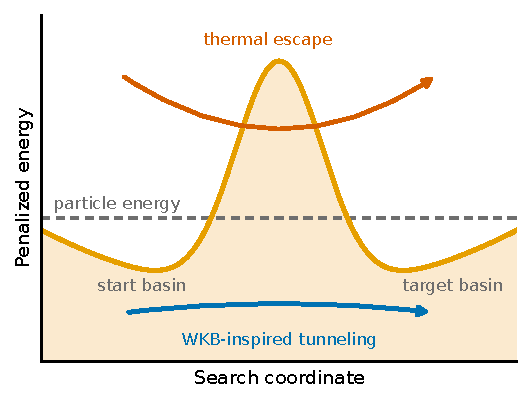
\includegraphics[width=\textwidth]{figures/tunneling_barrier_nature.pdf}
        \caption{Thermal escape versus tunneling-style escape.}
        \label{fig:tunnel_barrier}
    \end{subfigure}
    \hfill
    \begin{subfigure}[b]{0.47\textwidth}
        \centering
        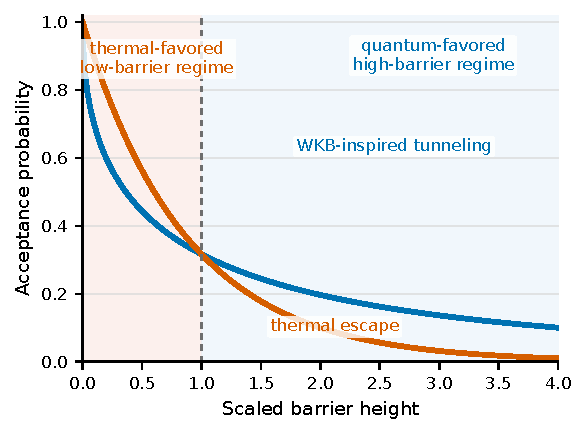
\includegraphics[width=\textwidth]{figures/tunneling_probability_nature.pdf}
        \caption{Acceptance profiles across increasing barrier height under a fixed effective jump width.}
        \label{fig:tunnel_probability}
    \end{subfigure}
    \caption{Conceptual schematic for the barrier-aware perturbation used in HP-PDHG. The right panel shows a one-dimensional slice in which the effective jump width and proportionality constants are absorbed into the horizontal scaling, so thermal escape decays as $\exp(-\beta h)$ while the WKB-inspired profile decays as $\exp(-\gamma \sqrt{h})$. The figure is intended as design intuition for the acceptance rule rather than as a claim of physical simulation.}
    \label{fig:tunneling_mechanism}
\end{figure}

Figure~\ref{fig:tunneling_mechanism} makes this distinction explicit. The left panel highlights the qualitative difference between surmounting a barrier and passing through it, while the right panel visualizes the fixed-width slice implied by \eqref{eq:tunnel_prob}. In the plotted schematic we set the two proportionality constants equal, so the crossover occurs at unit scaled barrier height. In the full algorithm, acceptance also depends on the proposal distance $\|x'-x\|$; the plotted curves therefore capture the correct functional trend rather than every degree of freedom in the multivariate rule.

\subsubsection{Multi-Scale L\'{e}vy Proposals}

When a non-local perturbation is triggered, proposals are generated from a mixture of proposal modes. History-guided moves interpolate toward elite incumbents, population-guided moves exploit directions suggested by the current ensemble, and random L\'{e}vy proposals provide heavy-tailed exploration that can jump between distant basins. The heavy-tailed component is especially important because Gaussian perturbations are too local to mimic barrier-crossing behavior in difficult feasibility landscapes. In practice, the proposal family is clipped to the bound box before acceptance is evaluated.

\subsection{Progressive Integrality Projection}
\label{subsec:measurement}

\subsubsection{Motivation}

Immediate rounding is often harmful in MIP because many coordinates are forced onto the integer lattice at once, often creating large primal violations. We therefore use progressive integrality projection, which lets the algorithm continue to benefit from the smooth geometry of the relaxation while gradually increasing discrete pressure.

\subsubsection{Cosine-Annealed Schedule}

The projection strength is controlled by
\begin{equation}
\lambda_t = \lambda_{\min} + \frac{\lambda_{\max} - \lambda_{\min}}{2}\left(1 - \cos\left(\pi \frac{t}{T}\right)\right),
\label{eq:measurement_schedule}
\end{equation}
where $T$ is the iteration budget. Early iterations have small $\lambda_t$, so the dynamics remain close to the continuous relaxation. Later iterations move $\lambda_t$ toward one, thereby shifting the search from exploration to discrete commitment.

\subsubsection{Soft Rounding Operator}

For each integer-constrained coordinate, we apply the soft-rounding map
\begin{equation}
\tilde{x}_j =
\begin{cases}
(1-\lambda_t)x_j + \lambda_t \operatorname{round}(x_j), & j \in \mathcal{I}, \\
x_j, & j \notin \mathcal{I}.
\end{cases}
\label{eq:soft_measurement}
\end{equation}
By Theorem~\ref{thm:measurement}, this operator contracts the integrality residual by a factor of $(1-\lambda_t)$ on every projected coordinate. The projection stage is therefore analytically interpretable rather than purely heuristic: it systematically reduces non-integrality while still leaving room for the repair stage to absorb small constraint violations.

\subsection{Feasibility-Aware Repair}
\label{subsec:repair}

Candidates generated by non-local perturbation or integrality projection are not accepted directly. Instead, they pass through a mixed-integer repair procedure that mirrors the current mainline implementation. The first stage clips variables to the bound box and rapidly repairs obvious binary violations by greedy flips. The second stage applies gradient-projection steps to the positive-part constraint residual, reprojects to the bounds, and rounds general integer coordinates after each candidate update. If this projected descent stalls, a local coordinate-descent pass is used as a fallback on the integer variables. A simpler projection-only repair routine is also available in the codebase, but the ablation and sensitivity studies reported here use the enhanced mixed-integer repair path. Repair is intentionally conservative: a candidate is promoted only if the final result satisfies the linear constraints, bounds, and integrality tests and remains competitive in objective value. This policy lets the algorithm explore aggressively at the candidate level while preserving a reliable incumbent set.

\subsection{Complete Algorithm}
\label{subsec:algorithm}

Algorithm~\ref{alg:quantum_pop_pdhg} summarizes the full procedure.

\begin{algorithm}[htbp]
\caption{HP-PDHG algorithmic workflow.}
\label{alg:quantum_pop_pdhg}
\begin{algorithmic}[1]
\REQUIRE Constraint matrix $A$, right-hand side $b$, objective $c$, bounds $l,u$, integer set $\mathcal{I}$, population size $K$, maximum iterations $T$, feasibility ratio $\eta$, feasibility weight $\omega_{\mathrm{feas}}$
\STATE Initialize population $\{(x^{(k)}, y^{(k)})\}_{k=1}^K$
\STATE Initialize best feasible solution $x^* \leftarrow \varnothing$
\STATE $T_1 \leftarrow \lfloor \eta T \rfloor$, $\omega \leftarrow \omega_{\mathrm{feas}}$
\FOR{$t = 1$ to $T$}
    \IF{$t = T_1 + 1$}
        \STATE $\omega \leftarrow 1$
    \ENDIF
    \FOR{$k = 1$ to $K$}
        \STATE Update $(x^{(k)}, y^{(k)})$ by one PDHG step
        \IF{$t \leq T_1$}
            \STATE Scale the dual state by $\omega$
            \STATE $\tau_{\text{measure}}^{(t)} \leftarrow \max(20,\lfloor \tau_{\text{measure}}/2 \rfloor)$
        \ELSE
            \STATE $\tau_{\text{measure}}^{(t)} \leftarrow \tau_{\text{measure}}$
        \ENDIF
        \IF{mod$(t, \tau_{\text{tunnel}}) = 0$}
            \STATE Sample tunneling proposal $x'$
            \IF{$x'$ is accepted by \eqref{eq:tunnel_prob}}
                \STATE $x^{(k)} \leftarrow x'$
            \ENDIF
        \ENDIF
        \IF{mod$(t, \tau_{\text{measure}}^{(t)}) = 0$}
            \STATE $\tilde{x} \leftarrow$ Soft\_Round$(x^{(k)}, \lambda_t)$
            \STATE $x^{(k)} \leftarrow$ Feasibility\_Repair$(\tilde{x})$
        \ENDIF
        \IF{$x^{(k)}$ is feasible and improves the incumbent}
            \STATE $x^* \leftarrow x^{(k)}$
        \ENDIF
    \ENDFOR
\ENDFOR
\RETURN $x^*$
\end{algorithmic}
\end{algorithm}

The practical interpretation of the algorithm is straightforward. PDHG provides a stable large-scale relaxation solver, the barrier-aware perturbation prevents the population from remaining confined to a single basin, integrality projection gradually contracts fractional coordinates, and repair plus incumbent screening preserves feasibility. The method is therefore not a collection of loosely connected heuristics, but a coordinated pipeline in which each component addresses a specific obstacle in moving from relaxation quality to integer-feasible incumbents.
